\documentclass[a4wide]{report}

\usepackage{amsmath}
\usepackage[a4paper, total={7in, 10.2in}]{geometry}
\usepackage{graphicx}
\usepackage[portuguese]{babel}
\usepackage[utf8]{inputenc}


\begin{document}

\noindent
{\bf Rafael V. Cacilhas  - Relatório 09 (\today)}

\vspace{0.5cm}

\section*{Exercício 1}

\subsection*{a) }

Dado o potencial u(r) = 
$\begin{cases} 
 4\epsilon \left[ \left(\frac{\sigma}{r}\right)^{12} - \left(\frac{\sigma}{r}\right)^6 + \frac{1}{4}      \right], r < r_c \\ 
 0, r > r_c
\end{cases} $
temos que a força $F = -\nabla u(r)$ é dada por:

\begin{equation}
F = \frac{\partial u(r)}{\partial r} = 24\frac{\epsilon}{\sigma} \left[ 2\left( \frac{\sigma}{r}\right)^{13} - \left(\frac{\sigma}{r}\right)^7     \right], r < r_c
\end{equation}

\begin{equation}
F = \frac{\partial u(r)}{\partial r} = 0, r > r_c
\end{equation}

Na Figura \ref{1a} estão representados os gráficos do potencial adimensional $u(r)/\epsilon$ e da aceleração $F/m_p$.

\begin{figure}[!htb]
\centering
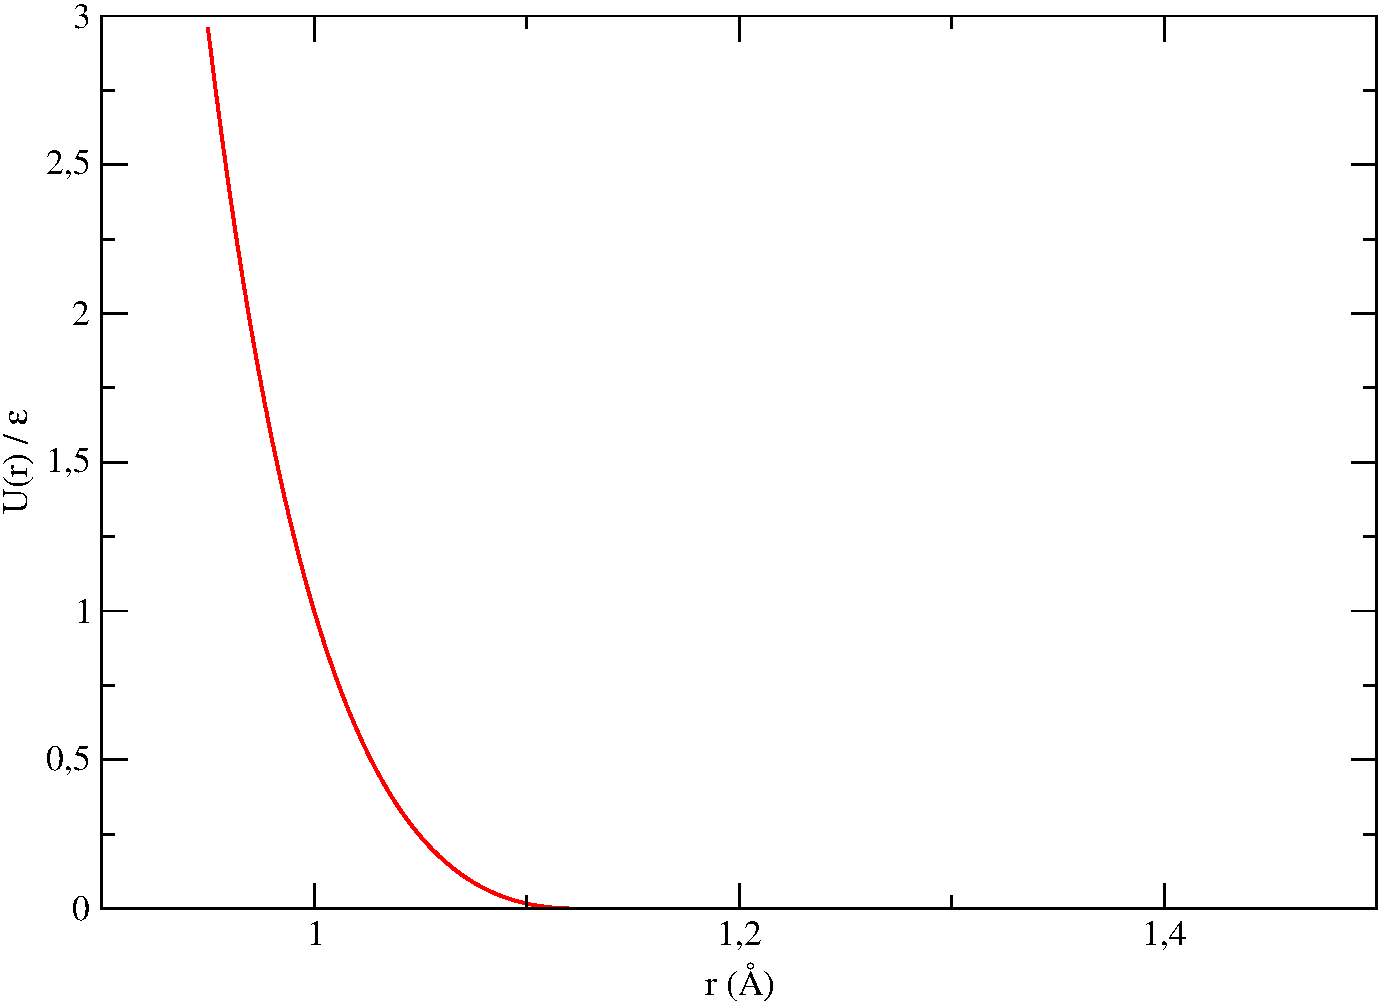
\includegraphics[width=0.4\textwidth]{U.pdf}
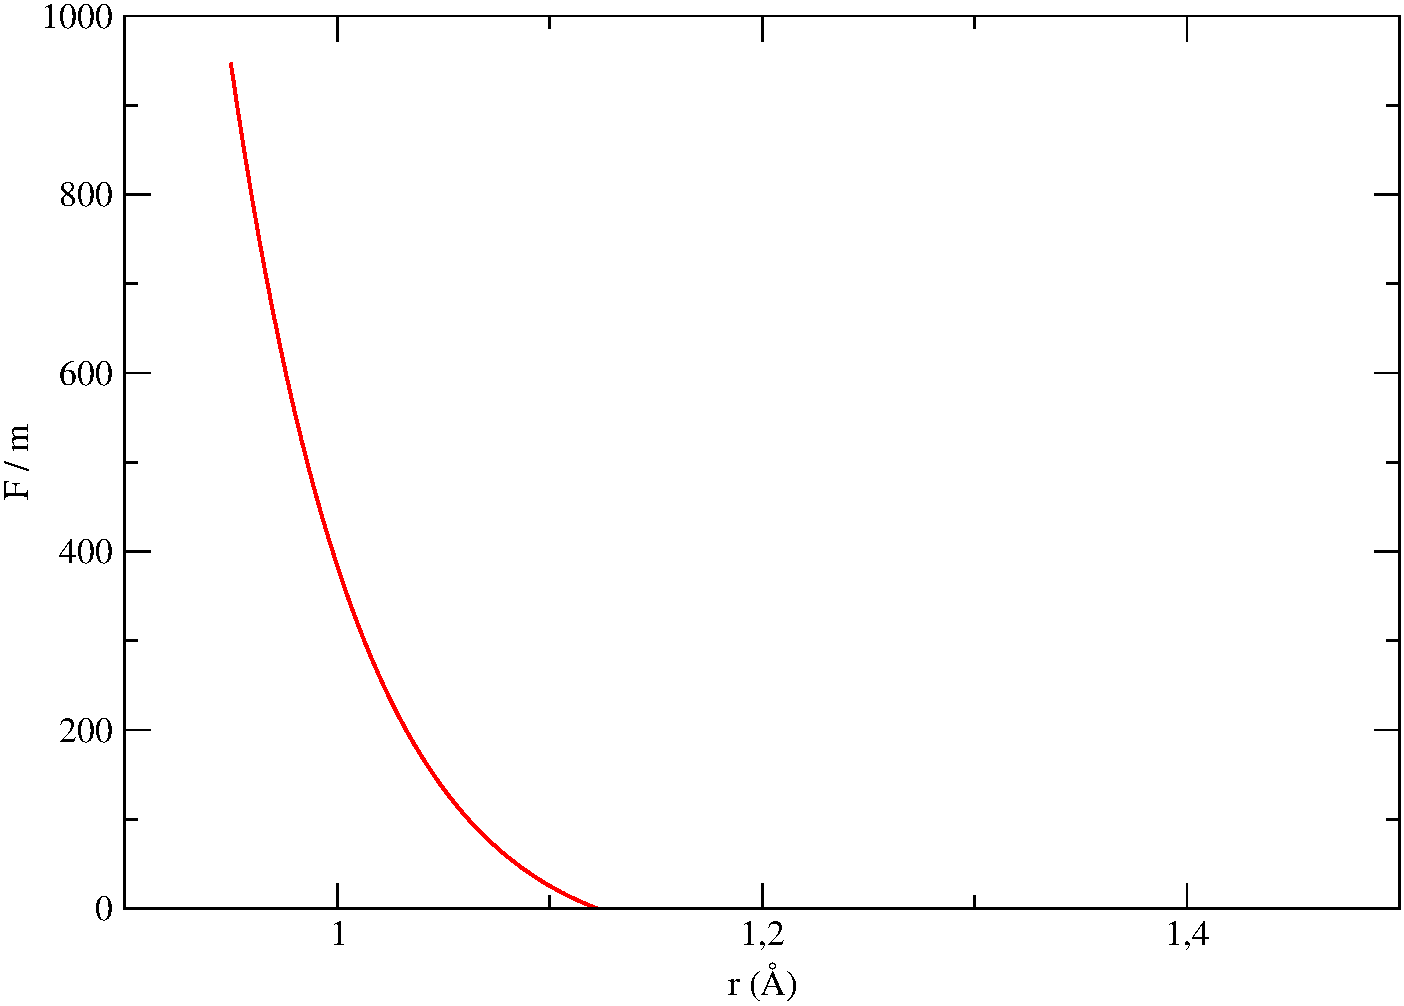
\includegraphics[width=0.4\textwidth]{forca.pdf}
\caption{Potencal adimensional (esquerda) e aceleração (direita) em função da distância.}
\label{1a}
\end{figure}
\end{document}


\subsection*{b) }
Sabemos  que as componentes da força $\vec{F_{kj}}$ são dadas por:

$\begin{cases} 
Fx = |F_{kj}|\cos\theta \\ 
Fy = |F_{kj}|\sin\theta
\end{cases} $

onde $\theta$ é o ângulo entre as particulas j e k.

Assim, podemos escrever
$\begin{cases} 
Fx = |F_{kj}|\frac{x_k - x_j}{|\vec{r}_k - \vec{r}_j|} \\ 
Fy = |F_{kj}|\frac{y_k - y_j}{|\vec{r}_k - \vec{r}_j|}
\end{cases} $


Ou, em termos do versor $\hat{r}_{kj} = \vec{r}_{kj}/|\vec{r}_{kj}|$ temos que para $r < r_c$:
\begin{equation}
Fx = 24\frac{\epsilon}{\sigma^2} \left[ 2\left( \frac{\sigma}{r_{kj}}\right)^{14} - \left(\frac{\sigma}{r_{kj}}\right)^8     \right](x_k - x_j), r < r_c
\end{equation}

\begin{equation}
Fy = 24\frac{\epsilon}{\sigma^2} \left[ 2\left( \frac{\sigma}{r_{kj}}\right)^{14} - \left(\frac{\sigma}{r_{kj}}\right)^8     \right](y_k - y_j), r < r_c
\end{equation}

E $Fx = Fy = 0$ caso $r > r_c$.


\subsection*{c) }

A configuração inicial do sistema e o histograma podem ser vistos na Figura \ref{2b1}.

\begin{figure}[!htb]
\centering
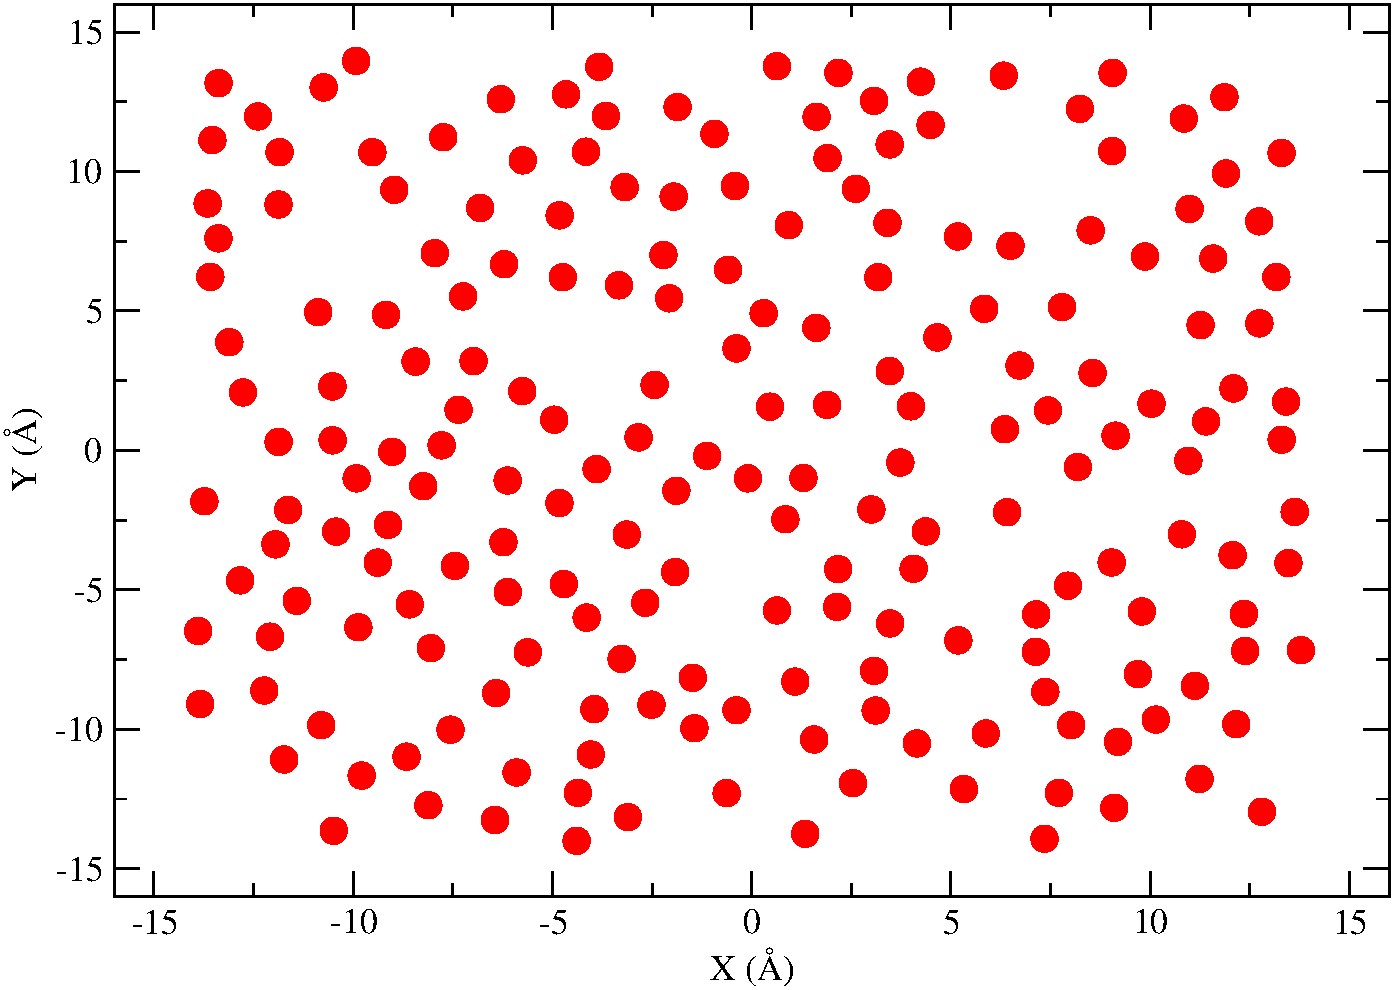
\includegraphics[width=0.4\textwidth]{mapa.pdf}
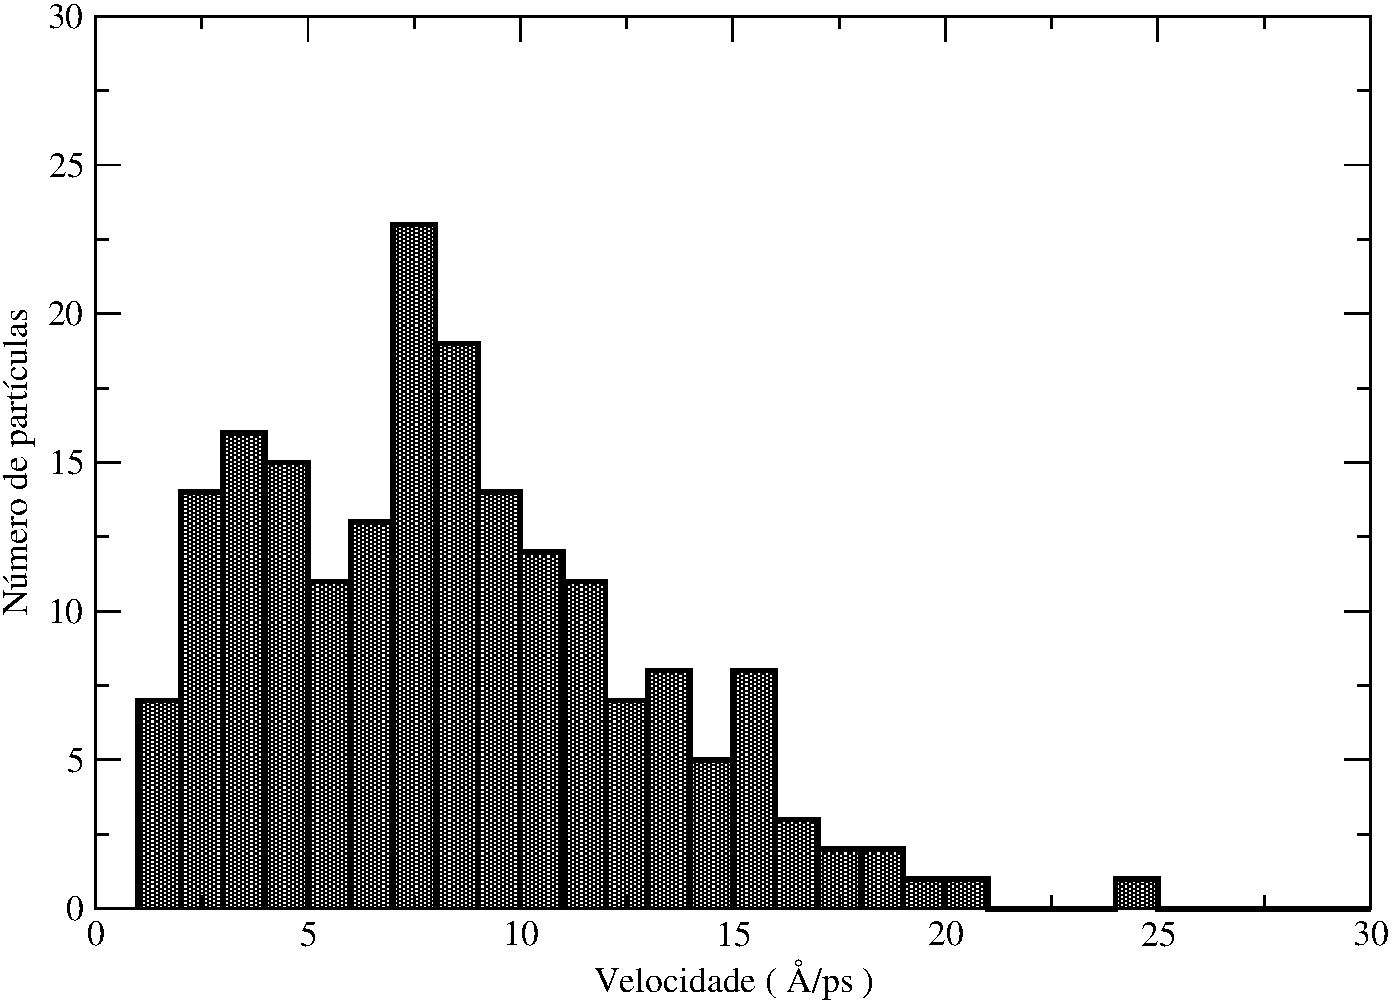
\includegraphics[width=0.4\textwidth]{hist.pdf}
\caption{Energias cinética, potencial e total para as condições iniciais 1.}
\label{2b1}
\end{figure}
\end{document}
